
\documentclass[journal]{IEEEtran}
    \usepackage[spanish]{babel}
    \selectlanguage{spanish}
    \usepackage[utf8]{inputenc}
    \usepackage{hyperref}


    % *** GRAPHICS RELATED PACKAGES ***
    %
    \ifCLASSINFOpdf
    \usepackage[pdftex]{graphicx}
    \DeclareGraphicsExtensions{.pdf,.jpeg,.png}
    \else

    \fi

    \usepackage{booktabs}
    \usepackage{tikz}
    \def\checkmark{\tikz\fill[scale=0.4](0,.35) -- (.25,0) -- (1,.7) -- (.25,.15) -- cycle;} 

    % *** MATH PACKAGES ***
    %
    \usepackage{amsmath}
    \usepackage{amsfonts}

    \interdisplaylinepenalty=2500

    \usepackage{array}

    \usepackage{fixltx2e}


    \usepackage{stfloats}
    \usepackage{dblfloatfix}

    \usepackage{booktabs}

    \usepackage{subcaption}

    % *** PDF, URL AND HYPERLINK PACKAGES ***
    %
    \usepackage{url}

    % correct bad hyphenation here
    \hyphenation{op-tical net-works semi-conduc-tor}


    \begin{document}
    %

    \title{Unconfused Terminator:\\ Red Neuronal desde cero para MNIST}
    %

    \author{Kenneth Obando Rodríguez,~\IEEEmembership{Instituto Tecnológico de Costa Rica}\\
            Alejandro Pacheco Quesada,~\IEEEmembership{Instituto Tecnológico de Costa Rica}}

    % The paper headers
    \markboth{Inteligencia Artificial, Mayo~2018}%
    {Shell \MakeLowercase{\textit{et al.}}: Bare Demo of IEEEtran.cls for IEEE Journals}

    % make the title area
    \maketitle

    
% :::::::::::::::::::::::
%     ABSTRACT
% :::::::::::::::::::::::
\begin{abstract}

\end{abstract}

% Note that keywords are not normally used for peerreview papers.
\begin{IEEEkeywords}
neural network, gradient descent, softmax, cross-entropy, relu, mnist, machine learning, image classification
\end{IEEEkeywords}

\IEEEpeerreviewmaketitle


\section{Introducción}
\IEEEPARstart{I}{}ndudablemente, poco a poco, el crecimiento y las utilidades que ofrece el área de Machine Learning han aumentado en gran escala. Es 
fascinante ver cómo la tecnología ha adoptado esta área de conocimiento para crear aplicaciones que facilitan o automatizan
muchas tareas. Sin embargo, para muchas personas el funcionamiento
de estas tecnologías es una caja negra y se tiene una idea errónea
de lo que realmente es lo que ``aprenden'' las máquinas y cómo lo hacen.
\par En este proyecto, se pretende romper esa barrera, y se quiere llevar a cabo la implementación de una red neuronal desde cero, de manera que sea posible entender, tanto desde el punto de vista matemático como computacional, cómo funcionan estos modelos de aprendizaje partiendo
de lo más básico, y cómo se da el proceso de aprendizaje mediante
técnicas como gradiente descendiente y \textit{backpropagation}. La red
que se desea implementar va a ser entrenada para clasificar imágenes con
dígitos escritos a mano.
\par La importancia de esto está en, posteriormente, tener una
idea clara de cómo funcionan estos modelos de aprendizaje y poder
implementarlos en otros tipos de problemas. Además, esto da paso
a poder utilizar \textit{frameworks} teniendo el conocimiento necesario para entender lo que está
sucediendo en esa caja negra y saber cómo podrían afectar diferentes cambios al modelo.


\section{Trabajo relacionado}
En este apartado, se citarán algunos trabajos realizados anteriormente en donde se proponen soluciones similares al problema de la investigación.
\par Si bien es cierto que el concepto de red neuronal no es algo que surgió recientemente, no es hasta hace poco tiempo que se han hecho implementaciones reales y prácticas, al punto de obtener tanta popularidad que han llegado a reemplazar algoritmos más antiguos muy usados. Antes del concepto de red neuronal, está detrás el concepto de perceptrón, que podría considerarse como una red neuronal de una única neurona. Este concepto fue mencionado por primera vez en \cite{Perceptron}, creado por Frank Rosenblatt. Debido a las limitaciones que tenía esta propuesta, tiempo después se sugiere la idea de crear capas con múltiples perceptrones. Una de las primeras menciones a esta idea aparece en \cite{percepBook}.
\par Actualmente, se han logrado buenos avances en Machine Learning utilizando diferentes arquitecturas de redes neuronales o variaciones de las mismas. Algunos ejemplos que caben mencionar son las redes de convolución \cite{convnet} y las redes neuronales recurrentes \cite{recnet}. 

\section{Metodología}
Para la resolución del problema y para las pruebas que se mostrarán más adelante, se deben considerar varios conceptos fundamentales: red neuronal, funciones de activación, 
función de pérdida y optimización por \textit{backpropagation}. La metodología consiste en implementar una red neuronal, o perceptrón multicapa, totalmente conectada (\textit{fully-connected}) para la clasificación de imágenes. Para ello, se requiere tener un vector de entrada, que será la capa de entrada. Además, se generan una o varias capas de diferente tamaño con neuronas (o perceptrones), las cuales corresponden a las capas ocultas, y finalmente, una capa de neuronas para la salida, que corresponden a la clasificación que predijo el modelo. Para el aprendizaje, lo que se busca es minimizar la función de pérdida respecto a los pesos $W$ de cada capa, que en esencia, constituyen los parámetros que determinan lo que sabe el modelo. Esta minimización del error se logra ajustando los pesos con \textit{backpropagation}. Con respecto a la clasificación y la activación, se hablará de ello con detalle más adelante. Cabe aclarar que para llevar a cabo este proceso, todas las funciones deben ser diferenciables. 
\par Respecto a los datos, se utilizará el set de datos MNIST. Este set contiene imágenes de $28x28$ píxeles en un solo canal, es decir, son en escala de grises. Este set posee diez clases distintas, que corresponden a los dígitos de las imágenes que se desean clasificar.
\par El lenguaje de programación utilizado fue Python y las operaciones de arreglos se simplificaron al utilizar la biblioteca Numpy.

\subsection{Entrenamiento y testing}
Se desea que la red a implementar sea capaz de reconocer dígitos escritos a mano, que serán pasados en forma de imagen a la red. Para esto, se utilizará el set de datos MNIST. Para el entrenamiento, se utilizarán todas las imágenes destinadas a entrenamiento que ofrece el set de datos, que corresponden a un poco más del 85\% del total de imágenes del set. Para las pruebas, MNIST también tiene un subconjunto de imágenes dedicadas a testing, que corresponden a un poco menos del 15\% del total.

\subsection{Red neuronal}
Constituye el modelo de aprendizaje que se entrenará para posteriormente realizar la clasificación de imágenes. Cada capa que constituye la red, exceptuando la de entrada, posee cierta cantidad de neuronas. Cada una de estas neuronas recibe un conjunto de entradas y para cada entrada hay un peso $W$ asociado. La red que se implementará en el proyecto tiene la siguiente arquitectura:

\begin{itemize}
    \item \textbf{Capa de entrada}: Esta capa corresponde al dato que se quiere clasificar con la red. El tamaño del vector de entrada será justamente el tamaño que tenga el dato. En el caso de esta investigación, al usar MNIST como set de datos, el vector de entrada tiene un tamaño de 784, que resulta del tamaño de cada imagen ($28x28$) visto en una sola  dimensión.
    \item \textbf{Capas ocultas}: Para la red neuronal que se implementará, se van a generar dos capas ocultas o intermedias. El tamaño de cada capa es variable y corresponde a un hyper-parámetro. Por lo tanto, el número de parámetros ($W$), varía según el tamaño de cada capa. 
    \item  \textbf{Capa de salida}: 
    Esta capa corresponde al clasificador de la red neuronal. Se utilizará una neurona por cada clase que tenga el set de datos utilizado. En este caso, al ser 10 clases distintas, la capa de salida tendrá 10 neuronas. Cuando finalmente se activan las neuronas de salida, se elige la que tenga la probabilidad más alta y ésta será la predicción hecha por la red para un dato dado.\\
\end{itemize}

Respecto a las neuronas que conforman las capas, es importante mencionar los siguientes aspectos:
\begin{itemize}
    \item \textbf{Pesos}: Inicialmente, por cada neurona de cada capa, se genera un peso aleatorio utilizando ``Xavier initialization'', que consiste en utilizar una distribución normal estándar para generar los pesos por cada capa. Posteriormente, cada uno de esos pesos es dividido por la raíz cuadrada del tamaño de la capa. Después de generar el primer set de pesos, eventualmente éstos se irán ajustando poco a poco para entrenar el modelo. 
    \item \textbf{Activaciones:} Por cada capa, las neuronas se conforman además de una función de activación que proporciona no linealidad a la red neuronal. Esta función puede ser distinta entre capas, y corresponde a un hyper-parámetro. 
\end{itemize}

\subsection{Forward y funciones de activación}
El \textit{forward pass} corresponde a la acción de clasificación. Se recibe un dato de entrada, en este caso una imagen, y se empieza a evaluar a través de toda la red neuronal. El procedimiento es el siguiente:\\
Para cada neurona $j$ de cada capa, se efectúa una pre-activación que corresponde a una función lineal de la forma \(f(X,W) = X\cdot W\), donde X es el vector de entrada formado por $x_i$ entradas y W es el vector de pesos para esa neurona, donde cada $w_i$ está asociado a una entrada. Entonces, finalmente se tiene una multiplicación de vectores de la forma: 
\begin{equation}\label{eq:linear}
    \sum_{i=1}^{m} x_i w_i
\end{equation}donde m es el tamaño de la entrada. Una vez calculada la pre-activación, ese resultado debe pasar por una función de activación, que da no linealidad a la red. Esto va a dar como resultado al final de la red, la clasificación para la entrada. Para la red implementada, se utilizaron dos funciones de activación distintas:
\begin{itemize}
    \item \textbf{Rectified Linear Units (ReLU)}: esta función de activación se utilizó para las dos capas ocultas de la red, y consiste únicamente en tomar el máximo entre el valor de entrada y 0. La función tiene la siguiente forma: 
    \begin{equation}\label{eq:relu}
        ReLU(x) = 
        \begin{cases}
        x & \text{if } x>0\\
        0 & \text{otherwise}
        \end{cases}
    \end{equation}
    \item \textbf{Softmax}: esta es la función de activación de la capa de salida. Se considera ideal para la última capa ya que esta función da una distribución de probabilidad para cada pre-activación. De esta manera, se estaría realizando la clasificación, y la salida que tenga la probabilidad más alta es la que el modelo considera como la clase perteneciente a la entrada. La función tiene la siguiente forma:
    \begin{equation}\label{eq:softmax}
        \forall \; k_i \in S\text{, }P(Y=K_i|X=x_i) = \frac{e^{S_{k_i}}}{\sum_{j}^{m} e^{S_j}}
    \end{equation}
    donde S corresponde al vector de pre-activaciones de la capa y cada $k_i$ sería una neurona. La sumatoria del denominador, corresponde simplemente a sumar todos los elementos del vector S.
\end{itemize}

\subsection{Función de pérdida: Cross-Entropy}

Parte de la función de pérdida utilizada para medir si el conjunto de pesos de la red cumple con los criterios de optimalidad. En otras palabras, esta función
proporciona el error del modelo de aprendizaje. Este error se ve reflejado en la capa de salida, al comparar la predicción con la clase real del dato. De esta forma, si la clase es incorrecta el error de la red va a aumentar en función de qué tan mal estuvo la predicción. Posteriormente, se deberá minimizar la función de error de manera que el modelo vaya aprendiendo. Para medir la pérdida, se utilizó la función Cross-Entropy. A continuación, se define la fórmula correspondiente:

\begin{equation}\label{eq:crossent}
L_i(S, y_i) = -log(P(Y=y_i|X=x_i))
\end{equation}
\[L_i(S, y_i) = -log(\frac{e^{S_{k_i}}}{\sum_{j}^{m} e^{S_j}})\]
donde el parámetro \(S\) corresponde al vector de activaciones de salida obtenidos al evaluar un dato \(x_i\) en la red neuronal, y el parámetro \(y_i\) corresponde a la etiqueta real del dato. 

Finalmente, la función de \textit{loss} completa, para medir la precisión del modelo con un conjunto de datos de prueba, tiene la siguiente fórmula:
\begin{equation}\label{loss}
L = \frac{1}{N} \sum_{i=1}^{N} Li( S, y_i)
\end{equation}
Donde \(N\) corresponde al total de datos de testing. 

\subsection{Dropout}
Consiste en, aleatoriamente, poner en cero los pesos de cierta cantidad de neuronas de una o ambas capas ocultas. Con esto se pretende que la red aprenda caminos alternativos para clasificar ciertas entradas, y así, evitar \textit{toverfitting}. Para la investigación, se realizarán ejecuciones con y sin \textit{dropout}. El \textit{dropout} se aplicó utilizando una distribución binomial con un $0.2$ de probabilidad.

\subsection{Gradientes y backpropagation}
El \textit{backpropagation} es quizás el proceso más importante de la implementación de la red neuronal. Este consiste en utilizar la gradiente de la función de error para ajustar todos los pesos de manera que minimicen el valor de la función (la pérdida). Esta gradiente se calcula respecto a los pesos de la red, pues es con quienes se desea minimizar el error. Esto puede observarse de la siguiente manera:
\begin{equation}\label{eq:grad}
    \forall \; w \in W, \;  \frac{\partial L}{\partial w}
\end{equation}

Donde $W$ hace referencia al conjunto de todos los pesos de la red. Esto significa que la gradiente surge de todos los pesos y posteriormente se usa realizar el ajuste. Una vez calculada la pendiente de Cross-Entropy con (\ref{eq:grad}), el ajuste para cada peso se realiza de la siguiente manera:

\begin{equation}\label{eq:ajuste}
    W^i = W^{i-1} - \alpha \nabla L
\end{equation}

Para $W^i$, la nueva matriz de pesos, $W^{i-1}$ la matriz de pesos de la iteración anterior y $\alpha$, un hyper-parámetro que establece la magnitud de la distancia entre $W^i$ y \(W^{i-1}\), conocido como \textit{learning rate}.


\section{Experimentos}

\subsection{Conjunto de Datos NMIST}
Para comprobar el funcionamiento de la red neuronal, se utiliza un conjunto de datos llamado NMIST \cite{NMIST}, que consiste en 60000 imágenes de dígitos escritos a mano debidamente etiquetados. Los dígitos se han normalizado y centrado en imágenes de $28 \times 28$ pixeles. Este conjunto de datos se recomiento para el aprendizaje de técnicas de machine learning y de reconocimiento de patrones. El mismo está dividido en un conjunto de entrenamiento de 60000 imágenes y otro conjunto de 10000 imágenes para realizar las pruebas.

Cada prueba se realiza con 30 epochs y batches de 32 imágenes, y se aplica diferentes configuraciones de red neuronal de dos capas y se registra los valores dados por la métrica de error CrossEntropy, y la precisión, tanto de los datos de entrenamiento como de prueba.

Se realiza un entrenamiento con sólo una capa con el fin de comparar su rendimiento respecto a la red con dos capas ocultas.

Además, se prueba la red neuronal utilizando una regularización de Dropout y se registra los valores obtenidos.

Para comprobar el funcionamiento se utilizan 10 números escritos a mano por el equipo de trabajo, estos números se pueden observar en la figura \ref{amano}. Se realiza el proceso de clasificación con la red neuronal ya entrenada.

\begin{figure}
    \centering
    \begin{subfigure}[b]{0.2\textwidth}
        
\includegraphics[width=\textwidth]{h0.png}
    \end{subfigure}
     %add desired spacing between images, e. g. ~, \quad, \qquad, \hfill etc. 
      %(or a blank line to force the subfigure onto a new line)
    \begin{subfigure}[b]{0.2\textwidth}
        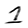
\includegraphics[width=\textwidth]{h1.png}
    \end{subfigure}
    ~
    \begin{subfigure}[b]{0.2\textwidth}
        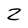
\includegraphics[width=\textwidth]{h2.png}
    \end{subfigure}
       \begin{subfigure}[b]{0.2\textwidth}
        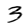
\includegraphics[width=\textwidth]{h3.png}
    \end{subfigure}
    
        \begin{subfigure}[b]{0.2\textwidth}
        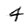
\includegraphics[width=\textwidth]{h4.png}
    \end{subfigure}
        \begin{subfigure}[b]{0.2\textwidth}
        
\includegraphics[width=\textwidth]{h5.png}
    \end{subfigure}
        \begin{subfigure}[b]{0.2\textwidth}
        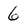
\includegraphics[width=\textwidth]{h6.png}
    \end{subfigure}
            \begin{subfigure}[b]{0.2\textwidth}
        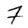
\includegraphics[width=\textwidth]{h7.png}
    \end{subfigure}
            \begin{subfigure}[b]{0.2\textwidth}
        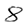
\includegraphics[width=\textwidth]{h8.png}
    \end{subfigure}
            \begin{subfigure}[b]{0.2\textwidth}
        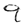
\includegraphics[width=\textwidth]{h9.png}
    \end{subfigure}
    \label{amano}
    \caption{Imágenes números hechos a mano por los estudiantes}\label{fig:animals}
\end{figure}


\section{Resultados}

\subsection{ Pruebas sin Dropout}
En el entrenamiento principal de la red, la métrica de error CrossEntropy se comporta de la forma esperada, disminuyendo su valor al inicio del entrenamiento considerablemente, luego baja su ritmo de error con varias osilaciones, Se obtiene el menor valor de error al finalizar los 30 epoch con un valor de 0.36 en el conjunto de datos de prueba (ver Figura \ref{crossentropySinDrop}).

Por otra parte, la precisión del modelo se mantiene relativamente estable, aunque mejorando con cada epoch. El proceso se inicia con un 86\% de precisión en el conjunto de prueba y llega a un máximo de 94\%(ver Figura \ref{precisionSinDrop}). 

\begin{figure}[!t]
\centering
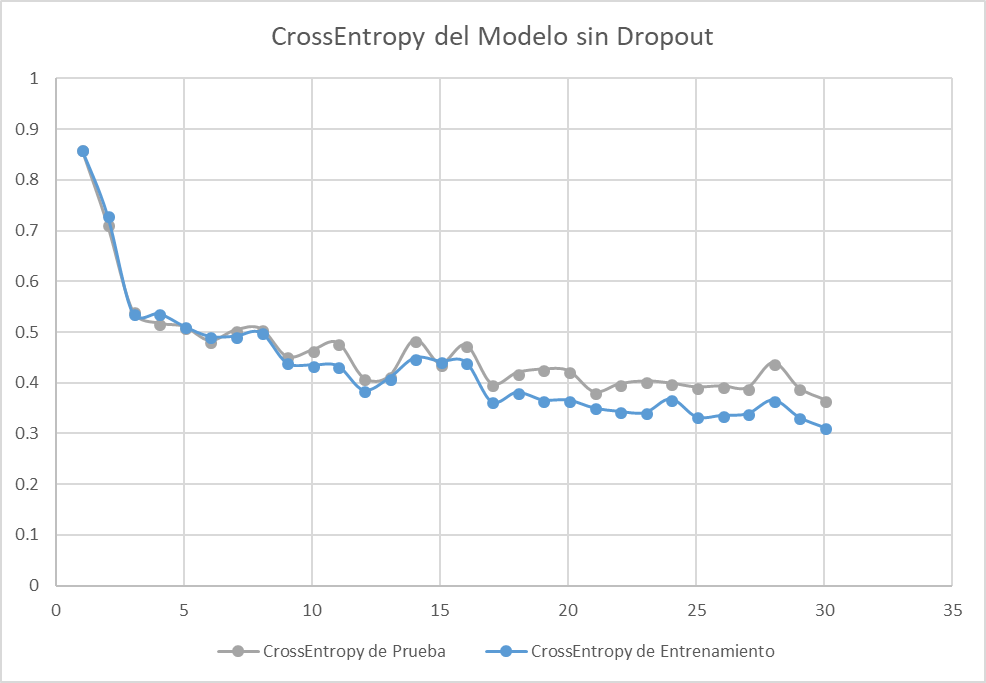
\includegraphics[width=3in]{crossentropySinDrop.png}
\caption{Valor de CrossEntropy calculado con NMIST por cada Epoch sin Dropout}
\label{crossentropySinDrop}
\end{figure}

\begin{figure}[!t]
\centering
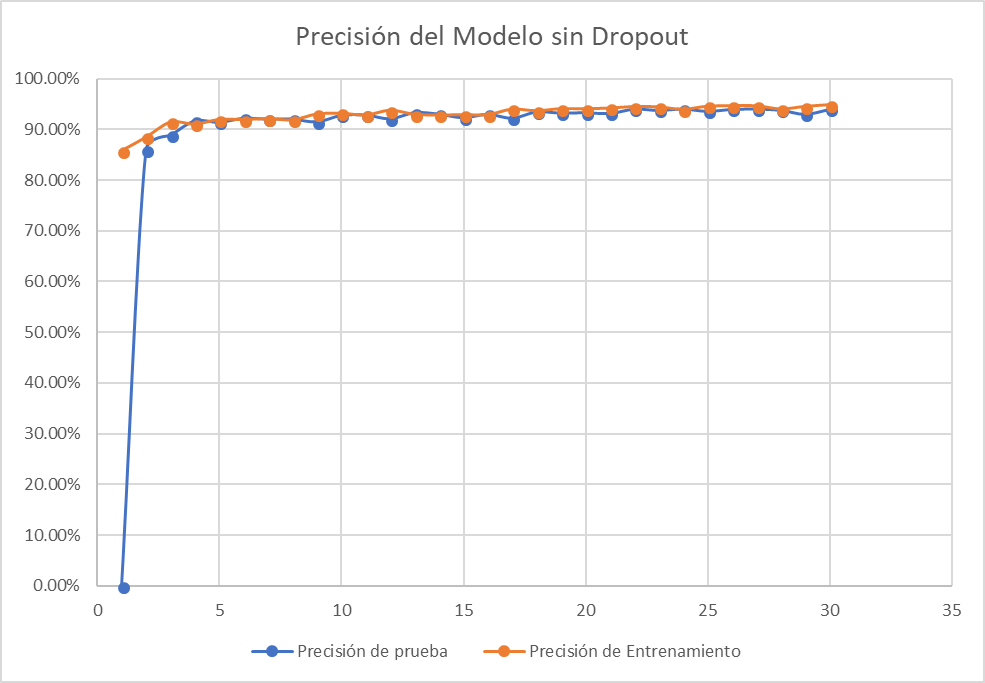
\includegraphics[width=3in]{precisionSinDrop.png}
\caption{Precisión obtenido con NMIST por cada Epoch sin Dropout}
\label{precisionSinDrop}
\end{figure}

\subsection{ Pruebas con Dropout}

Aplicando la regularización, se observa un comportamiento singular alrededor del epoch 8, donde la precisión del modelo mejora sustancialmente después de no lograr valores mayores a 0. En este mismo epoch, se observa un pico en el error de Crossentropy (ver Figura \ref{conDropout}).

La precisión es comparable con la obtenida sin el dropout, aunque más estable. Sospechamos que utilizando una cantidad mucho mayor de epochs, la red neuronal regularizada tendría un mejor rendimiento en comparación a una sin regularizar, gracias a esta misma estabilidad.

\begin{figure}[!t]
\centering
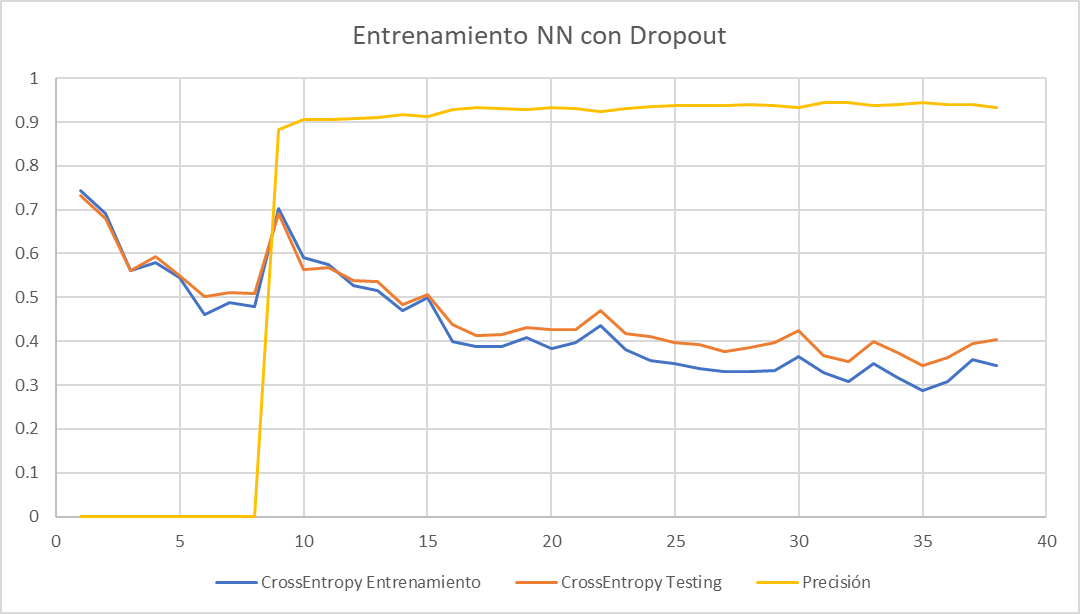
\includegraphics[width=3in]{conDropout.png}
\caption{Valor de CrossEntropy y precisión obtenidos con NMIST por cada Epoch con Dropout}
\label{conDropout}
\end{figure}

\subsection{ Pruebas con Números que no se encuentran en NMIST}

Al utilizar un conjunto de números propios, la red clasifica adecuadamente 4 de ellos. Este débil rendimiento, se debe a que estas imágenes no fueron tratadas con los mismo procedimientos que en NMIST (ver Cuadro 1).

\begin{table}[h]
\centering
\label{num1}
\begin{tabular}{@{}lll@{}}
\toprule
Dígito & Clasificación correcta      \\ \midrule
0      & \checkmark   \\
1      &                             \\
2      &                             \\
3      &                             \\
4      & \checkmark&  \\
5      &                             \\
6      & \checkmark   \\
7      &                             \\
8      &                             \\
9      & \checkmark   \\ \bottomrule
\end{tabular}
\caption{Clasificación de los números escritos por el equipo}
\end{table}



\section{Conclusión}

Esta investigación permite tener una idea general de las características de las redes neuronales y las posibilidades que permite a la hora de modelar la solución a un problema complejo, que por su gran cantidad de variables hace imposible diseñar un código estático \cite{Perceptrons}. 

Una de las principales conclusiones es la potencia computacional de una red neuronal, los modelos matemáticos empleados permiten aprovechar las características de paralelización y vectorización del hardware actual, además, pueden ser fácilmente adaptados a problemas abstractos obteniendo excelentes resultados.

Además, se ha observado como las Redes Neuronales son extremadamente versátiles, permiten incorporar una gran diversidad de parámetros y es por naturaleza modular. Esto lo coloca muy por encima de otras propuestas de aprendizaje como SVM, LASSO y PLS. 

La desventaja principal es que brinda poca información sobre qué variables afectan directamente la estimación, en otras palabras, no son modelos que permitan una interpretación de las variables. 

Por otra parte, gracias a esta investigación, se tiene evidencia empírica de que un batch de mayor tamaño permite un aprendizaje con menor oscilación y por ende, más estable, aunque el proceso se vuelve más lento que al realizarlo por cada imagen independiente.


\section{Trabajo a futuro}

Es una tarea pendiente implementar una red neuronal utilizando la librería CUDA, para utilizar los beneficios de un procesador gráfico GPU. Además, es una tarea pendiente investigar como variables multicorrelacionadas afectan la estimación de una red neuronal.
\cite{2014MachineLoss}

\ifCLASSOPTIONcaptionsoff
  \newpage
\fi

\bibliographystyle{IEEEtran}

\bibliography{mendeley_v2}

\section*{Anexos}


\begin{figure}[h]
    \centering
    \begin{subfigure}[b]{0.2\textwidth}
        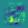
\includegraphics[width=\textwidth]{1}
    \end{subfigure}
     %add desired spacing between images, e. g. ~, \quad, \qquad, \hfill etc. 
      %(or a blank line to force the subfigure onto a new line)
    \begin{subfigure}[b]{0.2\textwidth}
        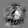
\includegraphics[width=\textwidth]{5}
    \end{subfigure}
    ~
    \begin{subfigure}[b]{0.2\textwidth}
        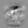
\includegraphics[width=\textwidth]{7.png}
    \end{subfigure}
       \begin{subfigure}[b]{0.2\textwidth}
        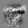
\includegraphics[width=\textwidth]{9.png}
    \end{subfigure}
    
        \begin{subfigure}[b]{0.2\textwidth}
        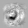
\includegraphics[width=\textwidth]{11.png}
    \end{subfigure}
        \begin{subfigure}[b]{0.2\textwidth}
        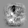
\includegraphics[width=\textwidth]{13.png}
    \end{subfigure}
        \begin{subfigure}[b]{0.2\textwidth}
        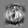
\includegraphics[width=\textwidth]{15.png}
    \end{subfigure}
            \begin{subfigure}[b]{0.2\textwidth}
        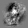
\includegraphics[width=\textwidth]{17.png}
    \end{subfigure}
            \begin{subfigure}[b]{0.2\textwidth}
        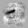
\includegraphics[width=\textwidth]{19.png}
    \end{subfigure}
            \begin{subfigure}[b]{0.2\textwidth}
        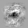
\includegraphics[width=\textwidth]{21.png}
    \end{subfigure}
    
    \caption{Imágenes de los pesos para la red entrenada NMIST}\label{fig:animals}
\end{figure}


\end{document}


